\documentclass{sig-alternate}
\usepackage{url}
\usepackage{pgffor}
\usepackage{tablefootnote}
\usepackage{multirow}
\usepackage{caption}
%\usepackage{subcaption}
\usepackage{subfigure}
\usepackage{comment}
\usepackage{graphicx}% http://ctan.org/pkg/graphicx
\usepackage[utf8]{inputenc}
\usepackage[usenames,dvipsnames,svgnames,table]{xcolor}
\usepackage{amssymb}
%\usepackage[]{algorithm2e}
\usepackage{algorithm}
\usepackage{algpseudocode}
\usepackage{tikz}
\usetikzlibrary{arrows, petri, topaths}
\usepackage{tkz-berge}

% Do-While
\algdef{SE}[DOWHILE]{Do}{DoWhile}{\algorithmicdo}[1]{\algorithmicwhile\ #1}%


\begin{document}

 \conferenceinfo{GECCO'15,} {July 11-15, 2015, Madrid, Spain.}
    \CopyrightYear{2015}
    \crdata{TBA}
    \clubpenalty=10000
    \widowpenalty = 10000

\title{A Study on Migration in the Heterogeneous Island Model}
%\subtitle{[Extended Abstract]
%\titlenote{A full version of this paper is available as
%\textit{Author's Guide to Preparing ACM SIG Proceedings Using
%\LaTeX$2_\epsilon$\ and BibTeX} at
%\texttt{www.acm.org/eaddress.htm}}}

\numberofauthors{4}
\author{
% You can go ahead and credit any number of authors here,
% e.g. one 'row of three' or two rows (consisting of one row of three
% and a second row of one, two or three).
%
% The command \alignauthor (no curly braces needed) should
% precede each author name, affiliation/snail-mail address and
% e-mail address. Additionally, tag each line of
% affiliation/address with \affaddr, and tag the
% e-mail address with \email.
\alignauthor
Krzysztof Nowak\\
       \affaddr{Advanced Concepts Team}\\
       \affaddr{European Space Agency (ESTEC)}\\
       \affaddr{Noordwijk, The Netherlands}\\
       \email{Krzysztof.Nowak@esa.int}
\alignauthor
Dario Izzo\\
       \affaddr{Advanced Concepts Team}\\
       \affaddr{European Space Agency (ESTEC)}\\
       \affaddr{Noordwijk, The Netherlands}\\
       \email{Dario.Izzo@esa.int}
\alignauthor
Daniel Hennes\\
       \affaddr{Advanced Concepts Team}\\
       \affaddr{European Space Agency (ESTEC)}\\
       \affaddr{Noordwijk, The Netherlands}\\
       \email{Daniel.Hennes@esa.int}
}

\maketitle
\begin{abstract}
Metaheuristics have proven to be an efficient method of handling difficult global optimization tasks.
State of art algorithms utilize several optimization techniques, allowing for occasional information exchange to leverage the trade-off between the exploration and exploitation.
Besides the popularity of metaheuristics among the evolutionary strategies researchers, there is also an interest in exploring parallel models of computation.
In this paper we focus at both concepts and analyze the performance of the heterogeneous island models and the impact of the selected hyper-parameters on the optimization performance.
We propose a methodology for characterizing the migration interplay between three metaheuristics, and evaluate the performance on real--parameter single objective optimization benchmarks.
%We observe a high sensitivity to both the frequency of migration and the migration strategies.

%heterogeneous metaheuristics
\end{abstract}

% A category with the (minimum) three required fields
% TODO: Find category
\category{H.4}{Information Systems Applications}{Miscellaneous}
%A category including the fourth, optional field follows...
%\category{D.2.8}{Software Engineering}{Metrics}[complexity measures, performance measures]

\terms{Global Optimization, Evolutionary Algorithms, Island Model, Parallel Computing, Parameter Tuning}

\keywords{Global Optimization, Evolutionary Algorithms, Island Model, Parallel Computing, Differential Evolution, Particle Swarm Optimization, CMA-ES}

\section{Introduction}
Search metaheuristics have been steadily growing in popularity over the recent years, mostly due to their performance in solving difficult optimization problems.
Although several search techniques are shown to perform well in global optimization, no single algorithm can claim to be universal~\cite{wolpert1997no}.
Popular algorithms, such as Differential Evolution (DE)~\cite{storn1997differential}, Particle Swarm Optimization (PSO)~\cite{james1995particle} or Covariance Matrix Adaptation Evolutionary Strategy (CMA-ES)~\cite{hansen2001completely},~\cite{hansen2003reducing} are often used as the building blocks of more sophisticated strategies for leveraging the exploration--exploitation trade-off using hybridization~\cite{Liao:2013:CEC}, adaptiveness~\cite{qin2009differential} or multiple restarts~\cite{auger2005restart}.
% TODO: Find example for PSO for either of those

% TODO: CEC WINNERS
%memetic~\cite{Lacroix:2013:CEC}, hybridization~\cite{Liao:2013:CEC}, restart strategies~\cite{EPFL-CONF-191267}.

% TODO: not increasing popular, its an old concept
Parallel metaheuristics are increasingly popular, mainly due to the shift in the processor development industry towards the multiple-core architectures, as well as the higher availability and lowering costs of the distributed computing services and platforms.
Several approaches to parallelization were proposed in the past~\cite{cantu1998survey}.%TODO: Add more examples of parallelization
In this paper we focus on the coarse-grained, multi-population parallelism known as the island model~\cite{cantu1999topologies}.
With the high customization and flexibility of the island model come the increasing number of hyper--parameters, which are difficult due to the already complex model.
One of the increasingly popular approaches is using several different metaheuristics on each island, and allowing for interplay between them in the form of migration.
Although such heterogeneous setup in algorithm's parameters has been shown to be effective~\cite{jjmorelo2014pool},~\cite{gong2011}, the heterogeneity in terms of distinct metaheuristics has been only partially explored.
The benefits of this type of hybridization in island model were reported only recently~\cite{izzo2012},~\cite{thiago2014}.
%best metaheuristics to interplay together in obtaining the final solution.
%Fine-tuning parameters of the island model for given problem is cumbersome, thus a 
% TODO: Find the bibtex for the Thiago guy

In this work we focus on the hybridization in terms of distinct metaheuristics, and provide the performance analysis with respect to the migration operator.
We propose a parametrization of migration rate and topology expressed in terms of migration probability, and investigate the interplay between selected hyper-parameters of the island model.
We show that CRAZY STUFF HAPPENS BUT IT IS GOOD.
%Structure of this paper is as follows

\textbf{Add Motivation}

\section{Experimental setup}
This section covers the details of our experimental setup, i.e. used metaheuristics, problems, experimental variables and performance evaluation.

\subsection{Metaheuristics}

The topic of our study were three stochastic and population-based optimization metaheuristics.
In this section we briefly explain each of them.%TODO: Fix this sentence

\subsubsection{Differential Evolution (DE)}
The Differential Evolution algorithm proposed by Storn and Price~\cite{storn1997differential} is a simple yet robust iterative search process.
The DE algorithm creates new individual by selecting a triple $\vec{x_1}, \vec{x_2}$ and $\vec{x_3}$ at random without replacement from the current population $P$, and computing:
%$$\vec{x_k} = F \cdot (\vec{x_1} - \vec{ + F \cdot (\vec{x_2} - \vec{x_3}),$$
$$\vec{x}_{i*}^{(t+1)} = \vec{x}_1^{(t)} + F \cdot (\vec{x}_2^{(t)} - \vec{x}_3^{(t)}),$$
with scaling factor $F=0.5$.
Solution $x_i^*$ replaces $x_i$ if $f(x_i^*) < f(x_i)$ (assuming minimization).

\subsubsection{Covariance Matrix Adaptation Evolutionary Strategy (CMA-ES)}

The CMA-ES proposed by Hansen et al.~\cite{hansen2001completely},~\cite{hansen2003reducing} optimizes the objective function by sampling $\lambda$ solutions ($i = 1,\ldots,\lambda)$ from the multivariate normal distribution:
$$x_i^{(t + 1)} = \textbf{m}^{(t)} + \sigma^{(t)} \cdot {\cal N}(0, {\cal C}^{(t)}),$$

where $\textbf{m}^{(t)}$, ${\cal C}^{(t)}$ and $\sigma^{(t)}$ denote mean, covariance matrix and step-size of the distribution at time $t$.
Out of $\lambda$ newly sampled and evaluated individuals, $\mu$ best are chosen and used for updating the parameters of the distribution.

\subsubsection{Particle Swarm Optimization (PSO)}

PSO is a bio-inspired stochastic search technique.
$$
    x_i^{(t+1)} = x_i^{(t)} + v_i^{(t)},
$$
where the velocity $v_i^{(t)}$ is updated as
$$
v_i^{(t+1)} = w(v_i^{(t)}) + c_1 \cdot \theta\cdot(pbest(x_i^{(t)}) - x_i^{(t)}) + c_2 \cdot \theta\cdot(gbest(x_i^{(t)}) - x_i^{(t)}).
$$

\subsection{Problems}

We test each hyper-parametrization setup on selected rotated variants of \emph{Sphere}, \emph{Discus}, \emph{Rosenbrock}, \emph{Schaffer F7}, \emph{Rastrigin} and \emph{Schwefel} functions, as proposed in the CEC 2013 benchmark suite (functions $f_1$, $f_4$, $f_6$, $f_7$, $f_{12}$ and $f_{15}$ respectively)~\cite{liang2013problem}.

\subsection{Heterogeneous Migration Model (HMM)}
Heterogeneous migration model described in this paper is in fact an island model, in which the concepts of \emph{topology} and \emph{migration rate} are unified in a single parametrization called \emph{migration probability}.
Migration rate $r$ and migration probability $p$ are two ways of parametrizing a single concept, i.e. the rate of information passing from one population to another (CITE TO Cantu PAZ about migration).
Although migration rate is a more popular parameterization, in this paper we will use the migration probability, as it allows for expressing ``fractional'' migration rates, e.g. for $p=0.75$, we can expect on average to migrate in $3$ out of $4$ possible synchronization points.
, and can be seen as reciprocals ($ 1/r \simeq p$).
%We allow HMM to have a migration rate dependent on the pair of islands exchanging information.
In HMM, probability of migration is dependent on the pair of populations exchanging the information.
This information can be stored as the weights in the directed acyclic graph of the model, thus replacing the global migration rate with a custom parameter determining the migration rate between any two populations.
For $n$ islands, the number of parameters modeling the probability of migration is equal to $n^2 - n$.
In reference to the island model, when $p_1=p_2=\ldots=p_{n^2-n}=c$ we obtain a fully--connected topology with the uniform ``migration rate'' equal to $\dfrac{1}{c}$ .
By setting some $m$ of those $n^2-n$ parameters to zero: $p_{k_1} = p_{k_2} = \ldots = p_{k_m} = 0$, we can obtain any other possible topology.
%Thus, HMM allows for more customization of the migration operator.

Because tuning such large space of parameters is very costly, we propose a reduced parametrization of HMM.
We assume that the probability of migration (directed edge) between given two \textbf{metaheuristics} is the same across the model, i.e. any two populations $P_i, P_j$ optimized by algorithms $H_k, H_l$ respectively, have the same probability of migration from $P_i$ to $P_j$ (see Figure~\ref{fig:2-4setup}).
This depends the number of parameters only on the number of distinct metaheuristics.

%We propose a setup with two metaheuristics running in parallel and allow for migration of the best solutions every generation with some probability $p_k$.
%We execute our two--island model synchronously, and allow for migration steps (every single generation).

\begin{figure}[htp]
\centering
\subfigure[$2$--heuristic, $4$--island setup ($4$ parameters)]{
    \label{fig:2-4setup}
    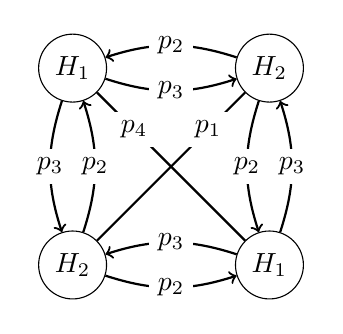
\begin{tikzpicture}[scale=2.5]
    \tikzstyle{vertex}=[draw,text=black,auto=left,circle,fill=white,minimum size=15pt]
    \tikzstyle{vertexred}=[draw,text=black,auto=left,color=red,circle,fill=white,minimum size=15pt]
    \tikzstyle{weight} = [fill=white]
    \tikzstyle{edge} = [draw,thick,->]
    \tikzstyle{edge2} = [draw,thick,-]

    \node[vertex] (a) at (1, 1) {$H_2$};
    \node[vertex] (b) at (0, 0) {$H_2$};
    \node[vertex] (c) at (1, 0) {$H_1$};
    \node[vertex] (d) at (0, 1) {$H_1$};

    \path[edge2] (a) to[near start] node[weight]{$p_1$} (b) ;
    \path[edge2] (c) to[near end] node[weight]{$p_4$} (d) ;
    %\path[edge] (b) to[bend right=18] node[weight]{$p_1$} (a);
    \path[edge] (a) to[bend right=18] node[weight]{$p_2$} (c) ;
    \path[edge] (c) to[bend right=18] node[weight]{$p_3$} (a);
    \path[edge] (b) to[bend right=18] node[weight]{$p_2$} (c);
    \path[edge] (c) to[bend right=18] node[weight]{$p_3$} (b) ;

    \path[edge] (a) to[bend right=18] node[weight]{$p_2$} (d) ;
    \path[edge] (d) to[bend right=18] node[weight]{$p_3$} (a);

    \path[edge] (b) to[bend right=18] node[weight]{$p_2$} (d);
    \path[edge] (d) to[bend right=18] node[weight]{$p_3$} (b) ;
    \end{tikzpicture}
}\quad
\subfigure[$3$--heuristic, $3$--island setup ($6$ parameters)]{

    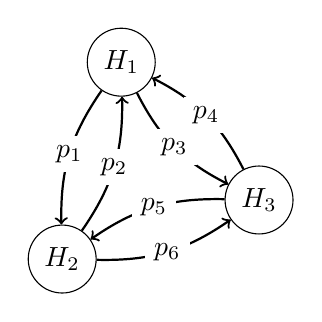
\begin{tikzpicture}[scale=2.5]
    \tikzstyle{vertex}=[draw,text=black,auto=left,circle,fill=white,minimum size=15pt]
    \tikzstyle{vertexred}=[draw,text=black,auto=left,color=red,circle,fill=white,minimum size=15pt]
    \tikzstyle{weight} = [fill=white]
    \tikzstyle{edge} = [draw,thick,->]
    \tikzstyle{edge2} = [draw,thick,-]

    \node[vertex] (a) at (0.3, 1) {$H_1$};
    \node[vertex] (b) at (0, 0) {$H_2$};
    \node[vertex] (c) at (1, 0.3) {$H_3$};

    \path[edge] (a) to[bend right=18] node[weight]{$p_3$} (c) ;
    \path[edge] (c) to[bend right=18] node[weight]{$p_4$} (a);

    \path[edge] (c) to[bend right=18] node[weight]{$p_5$} (b) ;
    \path[edge] (b) to[bend right=18] node[weight]{$p_6$} (c);

    \path[edge] (a) to[bend right=18] node[weight]{$p_1$} (b) ;
    \path[edge] (b) to[bend right=18] node[weight]{$p_2$} (a);

    \end{tikzpicture}
}
\caption{Examples of HMM setups}
\label{fig:setups}
\end{figure}

In our definition we use the following:
\begin{enumerate}
    \item $f$ -- optimized problem
    \item $\mathbb{P}$ -- A list of populations% instances with random initializations, in this paper we consider
        %$2 \leq |\mathbb{P}| \leq 8$
    \item $\mathbb{H}$ -- A list of metaheuristics, in this paper we consider
        $$\mbox{Domain}(\mathbb{H}) = \{\mbox{DE}, \mbox{PSO}, \mbox{CMA-ES}\}$$
    \item $h: \mathbb{P} \rightarrow \mathbb{H}$ -- an assignment of a metaheuristic to a population (many populations can be evolved by the same type of heuristic)
    \item $M: \mathbb{H} \times \mathbb{H} \rightarrow [0, 1]$ -- mapping from a pair of metaheuristics to the probability of migration% and a real value ranging from 0 and 1, modeling the probability of migration

\end{enumerate}

\begin{algorithm}
\caption{Main optimization procedure}
\label{alg:main_loop}
\begin{algorithmic}[1]
    \Procedure{Optimize}{$f, \mathbb{P}, h, M$}%\Comment{Single solution from population $P_1$ to $P_2$}
    \For{$P \in \mathbb{P}$}
        \State $P \gets \Call{Initialize}{f}$
    \EndFor
    \Do
        \For{$P \in \mathbb{P}$}
            \State $P \gets \Call{Evolve}{P, f, h(P)}$\Comment{Evolve population $P$, on a function $f$, using algorithm $h(P)$}
        \EndFor
        \For{$P_i, P_j \in \mathbb{P} \times \mathbb{P}, i\neq j$}\Comment{For each possible pair of populations}
            \State $x \sim U(0,1)$\Comment{Sample uniformly from $(0, 1)$}
            \If{$x < M(h(P_i), h(P_j))$}\Comment{Migrate if passed the probability threshold}\\
                \State $\Call{Migrate}{P_i, P_j}$
            \EndIf
        \EndFor
        \DoWhile{not $\Call{MeetsStopCriteria}{\mathbb{P}}$}
        \State $f_0, FE \gets \Call{GetResults}{\mathbb{P}}$\Comment{The best solution $f'$ and number of function evaluations $B'$}
\EndProcedure \mbox{ and }\Return $f_0, FE$
\end{algorithmic}
\end{algorithm}
The migration algorithm which we use is based on the ``best--replace--worst'' idea (CITE HERE), i.e. the incoming solution, if better than the worst solution in the population, will take its place (see Algorithm~\ref{alg:migr_1}).
\begin{algorithm}
\caption{Migration algorithm}
\label{alg:migr_1}
\begin{algorithmic}[1]
\Procedure{Migrate}{$P_1,P_2$}\Comment{Migrate from $P_1$ to $P_2$}
    \If{$\Call{Best}{P_1} < \Call{Worst}{P_2}$}\Comment{Assuming minimization}
        \State $\Call{Worst}{P_2} \gets \Call{Best}{P_1}$
    \EndIf
\EndProcedure
\end{algorithmic}
\end{algorithm}

    %Main drawback of this idea is the possibility of duplicating solutions in the population.
    %As long as $\Call{Worst}{P} > m$, the solution $m$ will be injected to population $P$.
    %This creates a problem as it effectively diminishes the population size -- intuitively, there is little gain in having duplicated information occupying a slot in the population.
    %We propose two variants of the algorithm~\ref{alg:migr_1} -- unique information filtering (Algorithm~\ref{alg:migr_3}) and fixed--index replacement (Algorithm~\ref{alg:migr_2}).
    %First variant adds a condition to the migration, such that the migrant coming from the population $P_1$ has to be unique within the receiving population $P_2$.
    %Verifying this condition introduces additional computational cost to the process.
    %Second variant avoids the problem entirely by assigning a fixed position in the population for all migrant solutions.
    %In such case the duplication is not possible, as the incoming duplicate $m$ would at most replace its previous instance at the fixed position.
    %This prevents only the ``direct'' duplication through migration process, as the population $P_2$ is free to create duplicates of $m$ in the meantime.
    %For this purpose we define a function $\Call{M-Idx}{P}$, which returns a reference to the ``migration'' slot in the population $P$.

\subsection{Methodology}

Since we treat each of the islands as a parallel computational unit, we assign a fixed budget of $20,000$ function evaluations for each of them.
We stop the execution if any of the following conditions are met:
\begin{enumerate}
    \item A solution within $10^{-8}$ from the global optimum is found
    \item The function evaluation budget is exhausted
    \item A population converges to a non-optimal point, i.e.\ the difference between the best and worst solution in the population is smaller than $10^{-12}$
\end{enumerate}

We repeat the experiment $1,000$ times, obtaining a pool of independent runs, each of those could either be successful (condition 1 above) or unsuccessful (condition 2 or 3).
Each run can either a) find an optimal solution (successful run), b) exhaust the budget before arriving at a solution or c) converge to a local optimum (unsuccessful runs).

\subsection{Uniform migration experiment}
This section presents the core idea and methodology used in this paper, as well as serve as an introduction to our subsequent exhaustive experiment.
In this and the following experiments we will observe the behaviour of selected metaheuristics with respect to the migration operator.
We do not focus on the convergence rate, instead we analyze the running time distributions and expected running time (expected number of function evaluations to global minima convergence).

Let consider a two--island setup, where each population is evolved using two distinguished instaces of Differential Evolution algorithm running synchronously (denoted as H$_1$ and H$_2$).
To get a better understanding of the effect of migration we will not actively observe the island running algorithm DE$_1$, i.e. the stopping criteria and the number of function evaluations are considered and measured only locally for DE$_2$.
We will iterate over the probability of migration from algorithm H$_1$ to H$_2$ (parameter $p_1$), and consider two cases for the opposite (parameter $p_2$): 
\begin{enumerate}
    \item $p_2$ is always equal to 0 -- island DE$_2$ does not send any solutions to DE$_1$
    \item $p_2$ is equal to $p_1$ -- island DE$_2$ will send solutions to DE$_1$ with the same probability
\end{enumerate}
Figure~\ref{graph:twoisl} presents the experimental setup on a diagram.
\begin{figure}[ht!]
    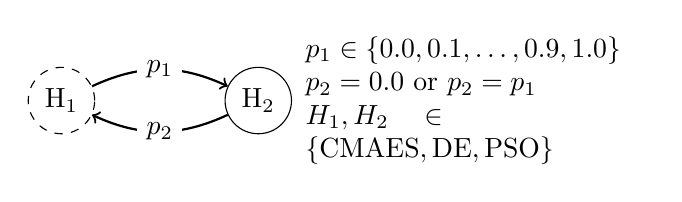
\begin{tikzpicture}[scale=2.5]
    \tikzstyle{vertex}=[draw,text=black,auto=left,circle,fill=white,minimum size=24pt]
    \tikzstyle{vertexred}=[draw,text=black,auto=left,color=red,circle,fill=white,minimum size=15pt]
    \tikzstyle{weight} = [fill=white]
    \tikzstyle{edge} = [draw,thick,->]
    \tikzstyle{edge2} = [draw,thick,-]

    \node[vertex, dashed] (a) at (0, 0) {H$_1$};
    \node[vertex] (b) at (1, 0) {H$_{2}$};


    \node[text width=4.3cm] at (2.1, 0.0) {%$H = \{\mbox{DE}, \mbox{CMAES}\}$\\
        $p_1 \in \{0.0, 0.1, \ldots , 0.9, 1.0\}$\\
        $p_2 = 0.0 \mbox{ or } p_2 = p_1$\\
        $H_1,H_2 \in \{\mbox{CMAES},\mbox{DE},\mbox{PSO}\}$};

    \path[edge] (a) to[bend left=25] node[weight]{$p_1$} (b) ;
    \path[edge] (b) to[bend left=25] node[weight]{$p_2$} (a);

    \end{tikzpicture}
    \label{graph:twoisl}
    \caption{Two--island setup with both algorithms running synchronously and migrating with probabilities $p_1$ and $p_2$. We observe only the results of H$_2$.}

\end{figure}
In the following parts of this section we will focus on investigate the particular properties of several metaheurstics 

\subsubsection{Differential Evolution (DE)}

%\begin{table*}
%    \label{table:pkvalues}
%    \begin{tabular}{|c|c|c|c|c|c|c|c|c|c|c|}
%        \hline
%        Seeder & $f_1$   & $f_4$ & $f_6$ & $f_7$ & $f_9$ & $f_{12}$ & $f_{13}$ & $f_{15}$ & $f_{16}$ & $f_{20}$ \\\hline
%        DE     & B (1.0) & B (1.0) & B (1.0) &  &  &  &  &  &  &  \\
%        CMAES  & N       &  &  &  &  &  &  &  &  &  \\
%        PSO    & B (1.0) &  &  &  &  &  &  &  &  &  \\
%    \end{tabular}
%    \caption{Cooperation for DE}
%\end{table*}

To present the key ideas of our methodology on an example, let us take a closer look on a setup with the algorithm DE optimizing the problem $f_7$, while being sent solutions from DE, CMAES and PSO.
First, let us look at the distribution of running times of single and independent runs of CMAES, DE and PSO on problem $f_7$ (see Figure~\ref{fig:distr_cmaes_jde_7}).
It is quite clear that on this particular problem, CMAES converges to global minimum much faster than DE, while PSO is significantly slower than the remaining two algorithms.
Let us consider $H_1 = \mbox{DE}, H_2 = \mbox{DE}$, and analyze the change of the distribution of $H_2$ over varying parameters $p_1$ and $p_2$.
Figure~\ref{fig:single_jde_jde_7} presents the distribution of $10,000$ resampled running times (approximated by a Gaussian kernel density estimation) as shown in Algorithm~\ref{alg:resample}.
\begin{figure}[ht]
  \centering
  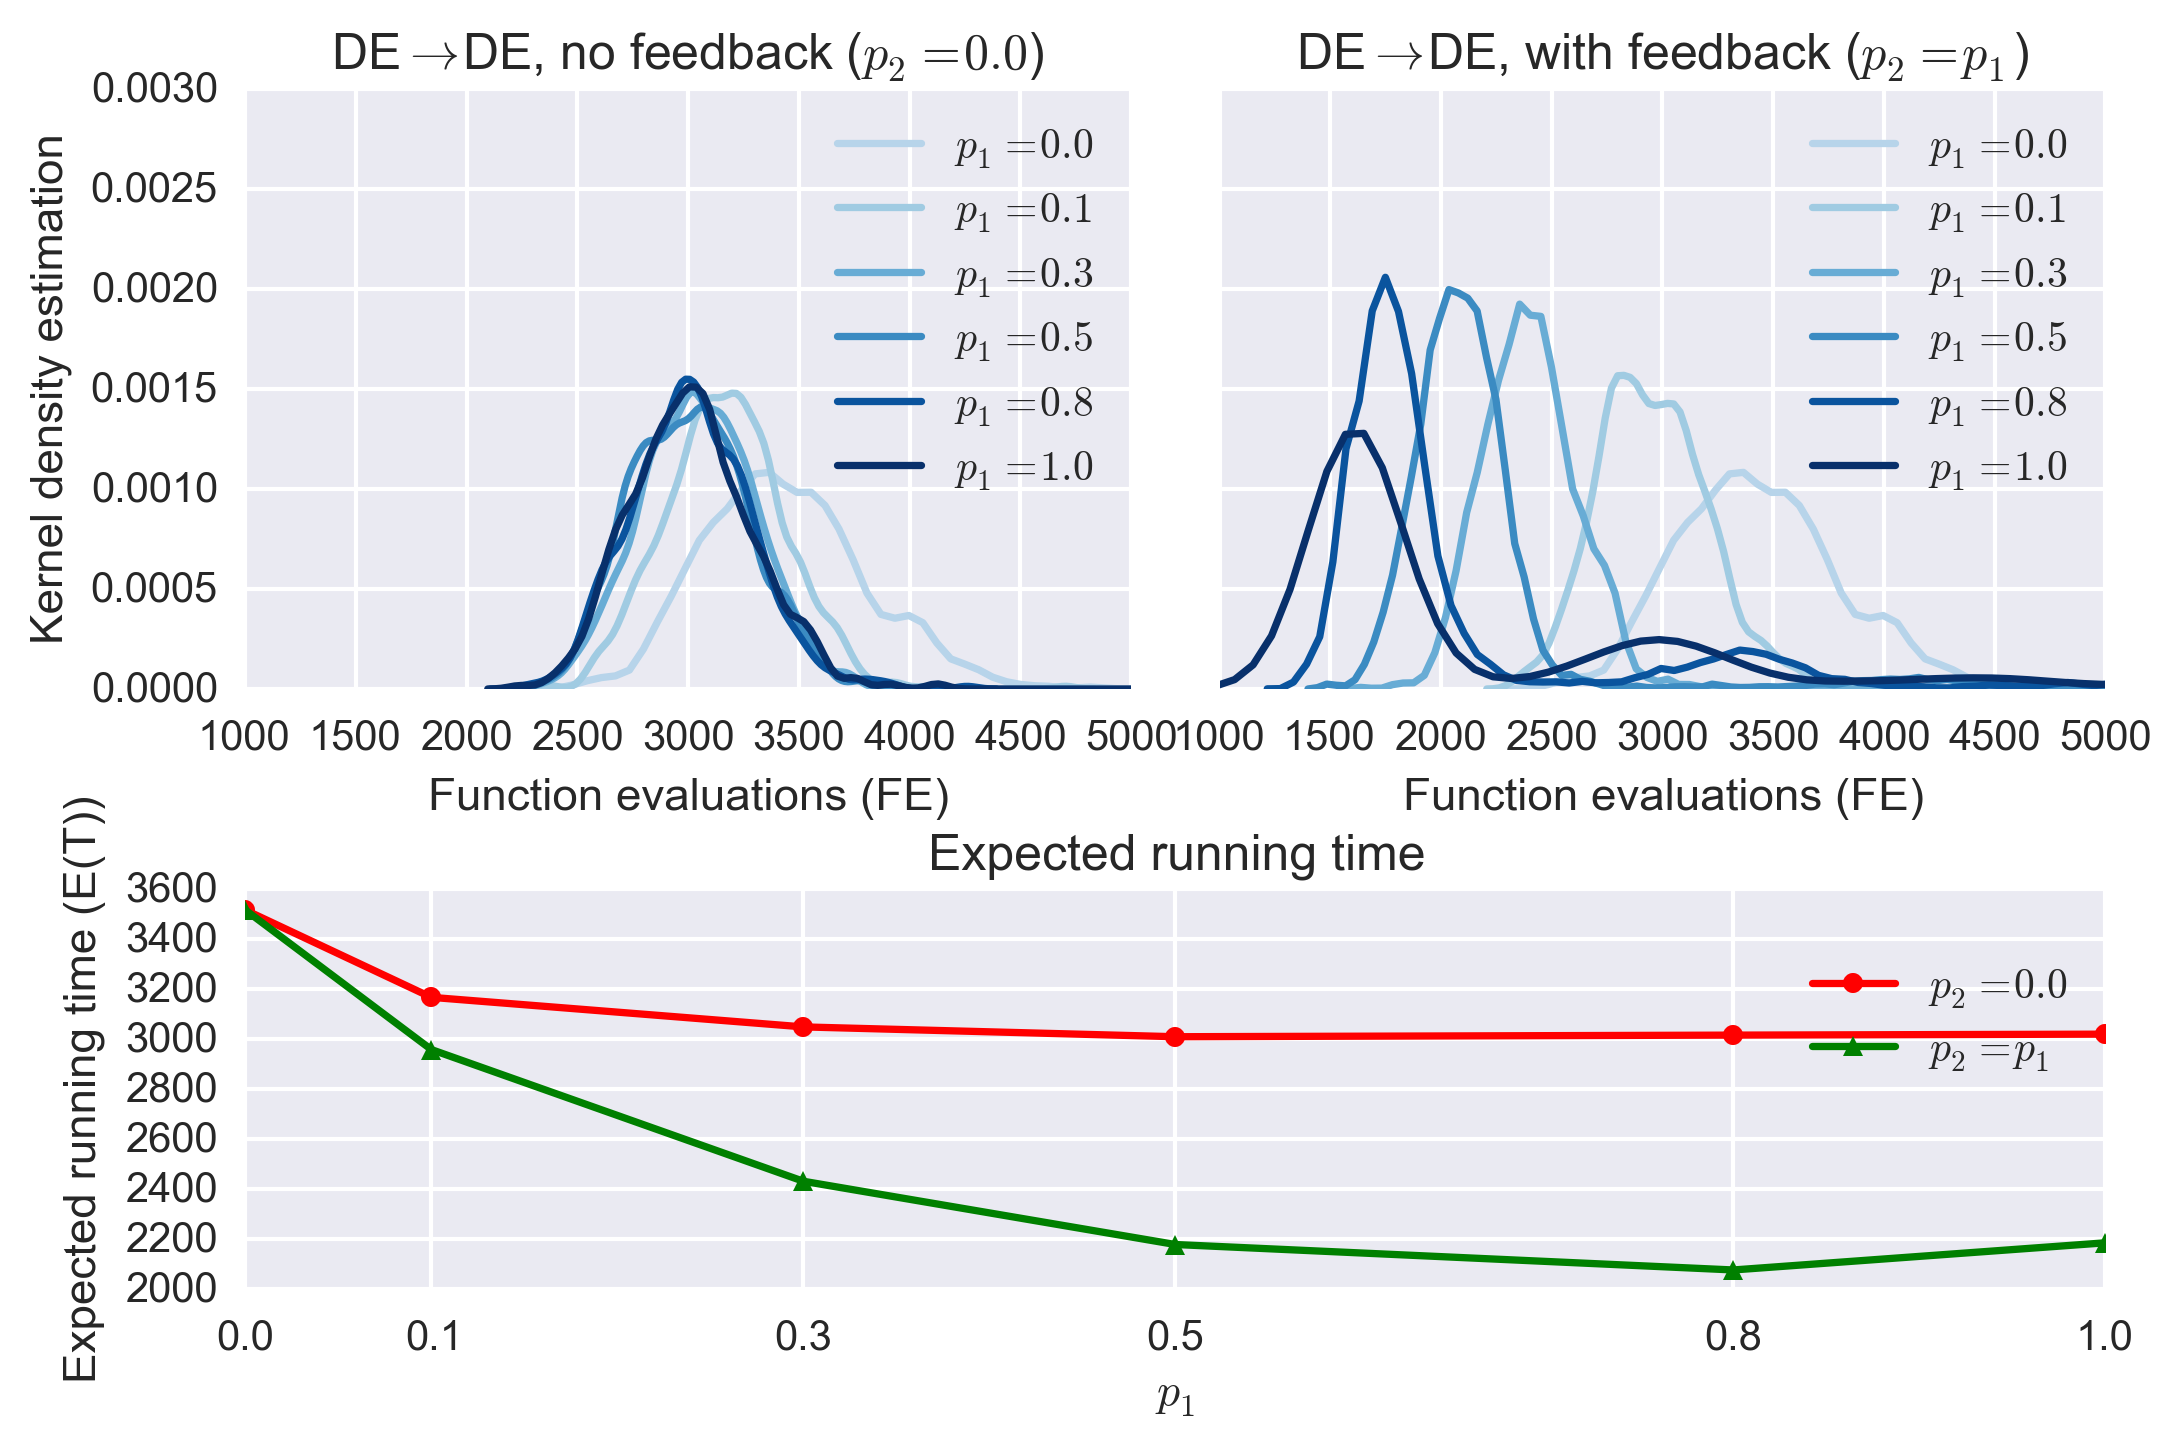
\includegraphics[width=\columnwidth]{figures/single_jde_jde_cec_7.png}
  \label{fig:single_jde_jde_7}
 \caption{Running time behaviour of homogeneous 2--island DE/DE setup on problem $f_{12}$.}
\end{figure}

Two plots at the top present the case where $p_2 = 0$ (left), and $p_1 = p_2$ (right), describing the one--directional and two--directional migrations respectively (occasionally we will refer to latter as the \emph{feedback} case).
%For one--directional case, the migration has a positive effect, lowering the expected running time with the higher value    $p_1$ increases until migration every single generation ($p_1 = 1.0$).
By allowing for migration with probability $p_1 = 0.1$ the mean shifts from $3,360$ to $3,100$ function evaluations, yet after the initial speedup the distribution and the expected running time change very little once $p_1 >= 0.3$.
In the feedback scenario, not only we notice a significant speedup compared to one--directional case, but we observe a continuing trend with the improving expected running time until $p_1 = 1$ (migration every generation).
This shows that migration, even when observed strictly from the perspective of the ``receiver'', is not a one--directional process, and can be reinforced by mutual information exchange.

Let us modify our experiment and instantiate the ``sending'' island with the algorithm CMAES ($H_1$).
Both algorithms are run synchronously and as before we will monitor only the distribution and stopping criteria for population evolved by an instance of DE ($H_2$).
\begin{figure}[ht]
    \centering
    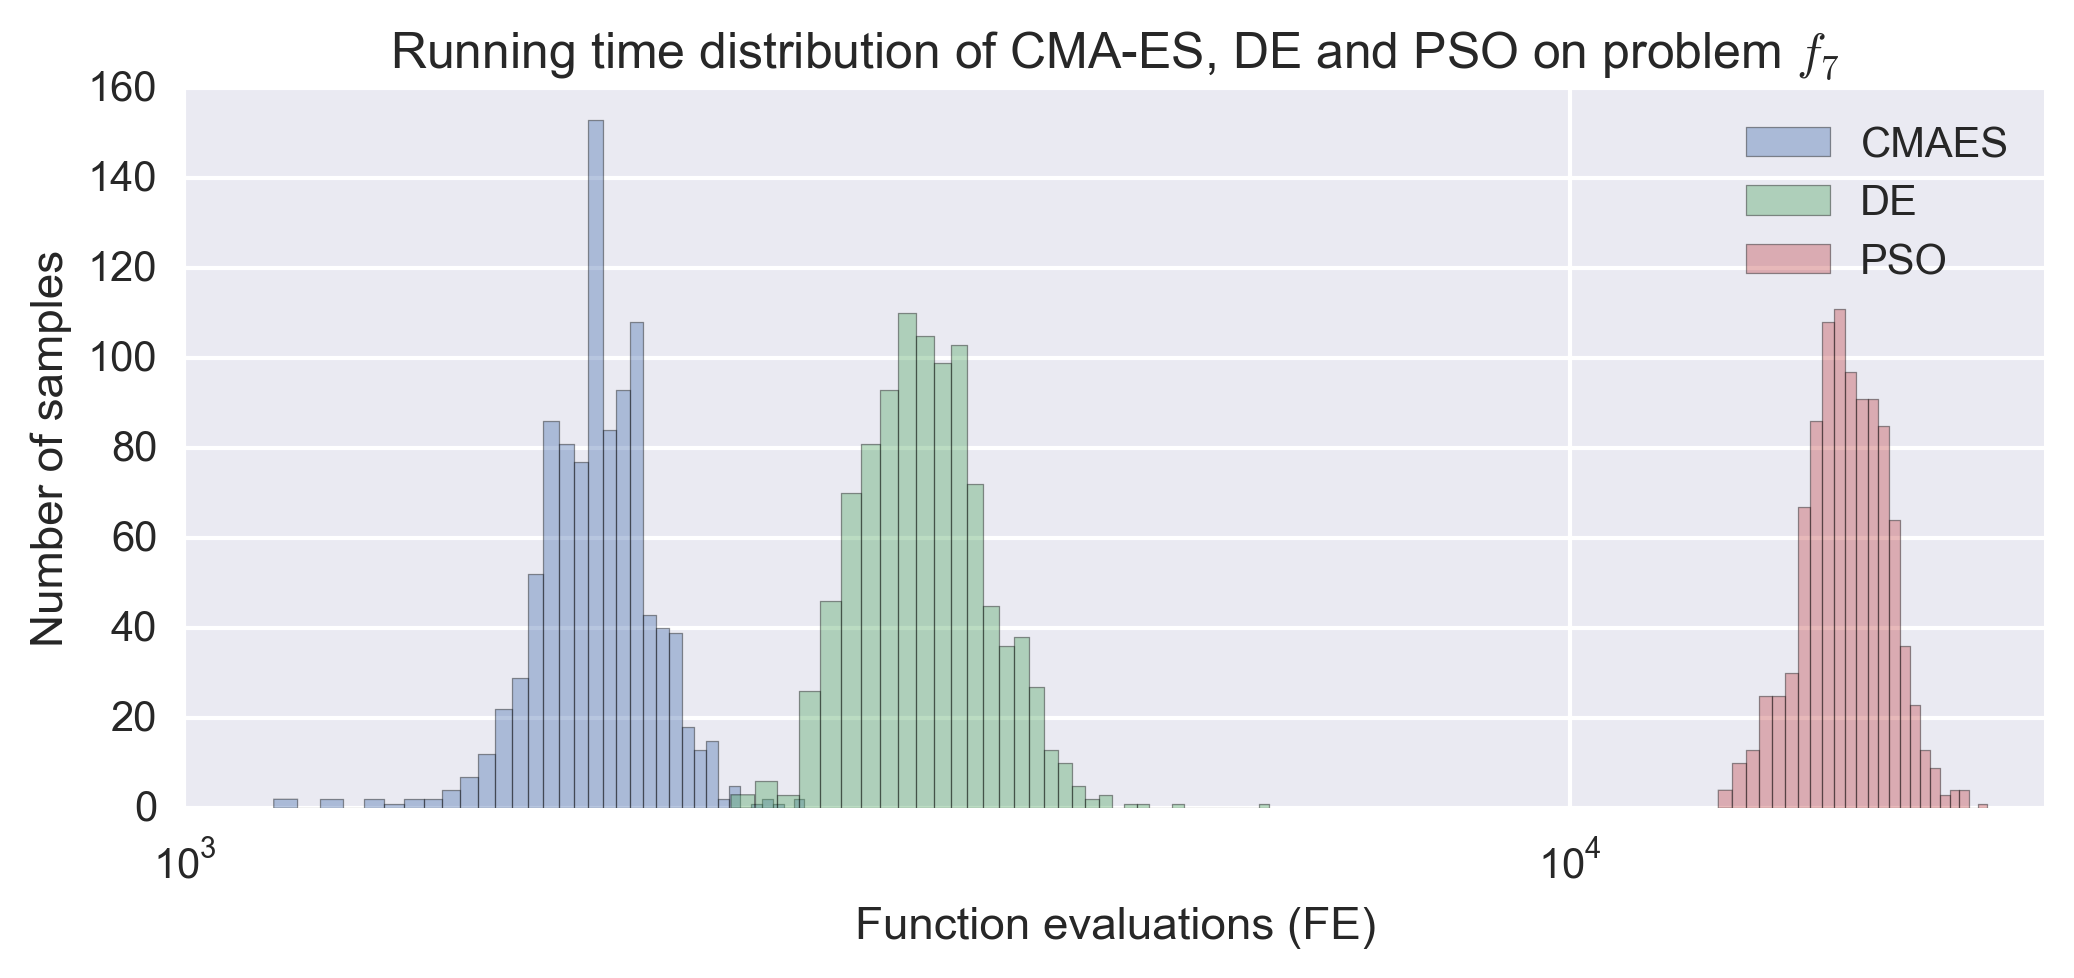
\includegraphics[width=\columnwidth]{figures/single_distr_7.png}
    \label{fig:distr_cmaes_jde_9}
    \caption{Distribution of running times for algorithms CMA-ES and DE on problem $f_9$.}
\end{figure}
Not surprisingly, for one--directional injection from CMAES to DE (see Figure~\ref{fig:single_cmaes_jde_9}), we observe a significant improvement in the running time distribution (mean shift from $3,360$ to $2,120$).
\begin{figure}[ht]
  \centering
  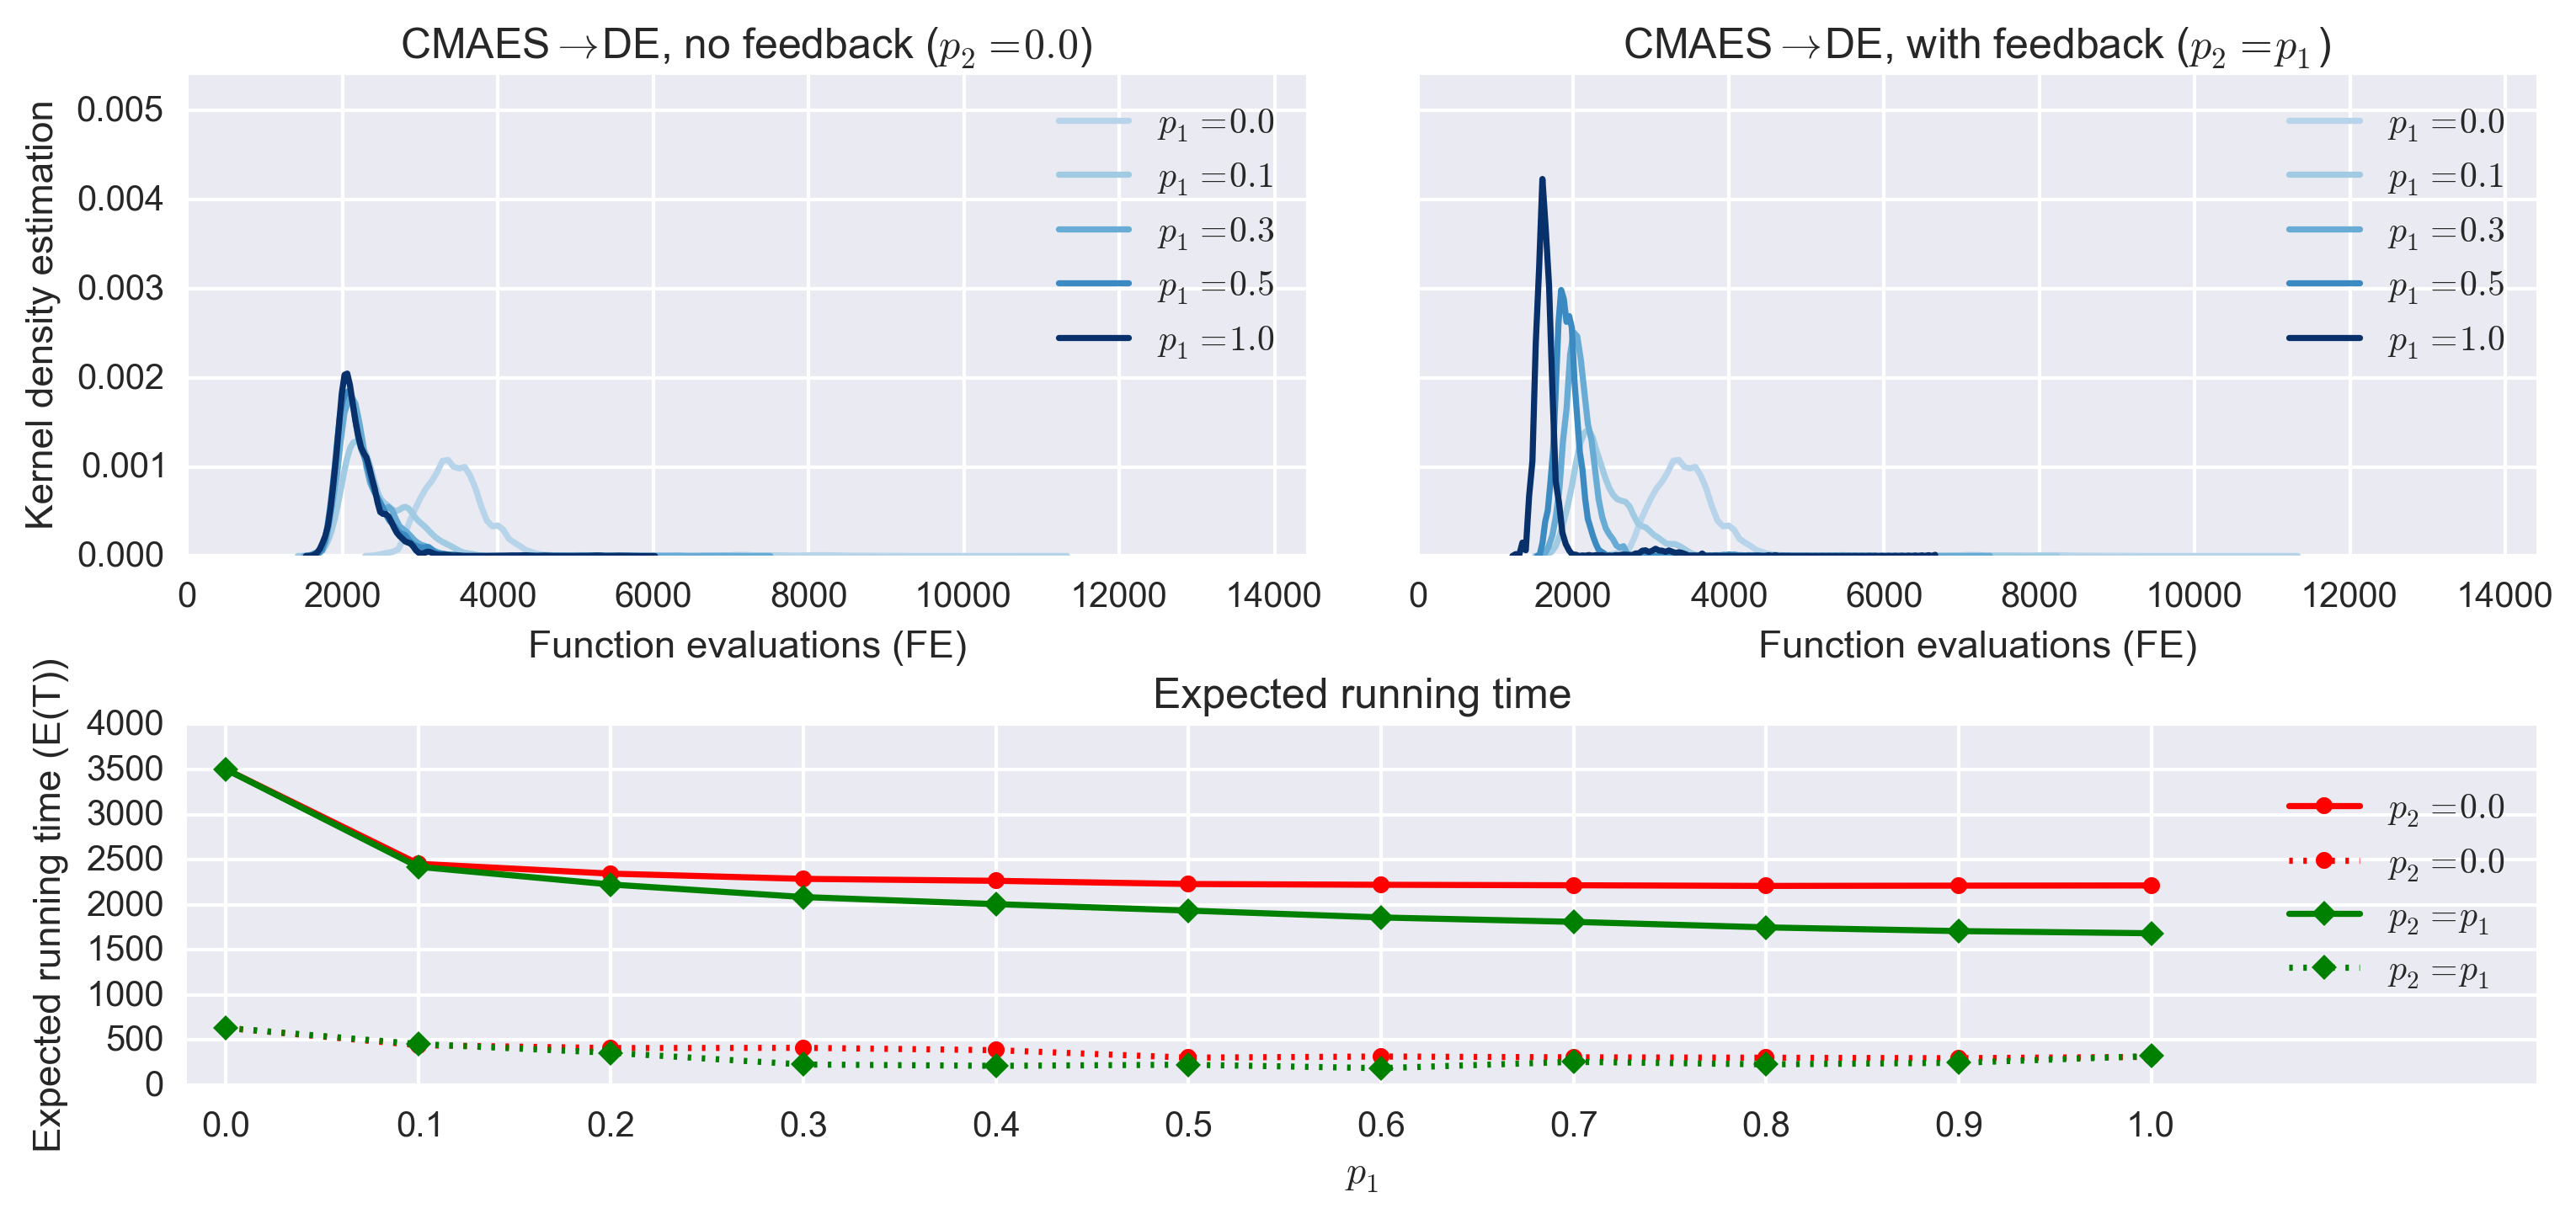
\includegraphics[width=\columnwidth]{figures/single_cmaes_jde_cec_7.png}
  \label{fig:single_jde_jde_7}
 \caption{Running time behaviour of homogeneous 2--island DE/DE setup on problem $f_{12}$.}
\end{figure}
As before, the probability of migration in one--directional setup starts to reach its limit as soon as $p_1 > 0.3$, however, when $p_2 = p_1$, we notice a gradual improvement of expected running time until $p_1=p_2=1.0$.
It is worth noting that even though we had previously established CMAES as being ``faster'' algorithm on problem $f_9$, the feedback from the ``slower'' DE was overall beneficial.

Finally, let us observe the scenario where $H_1 = \mbox{PSO}$.
\begin{figure}[ht]
  \centering
  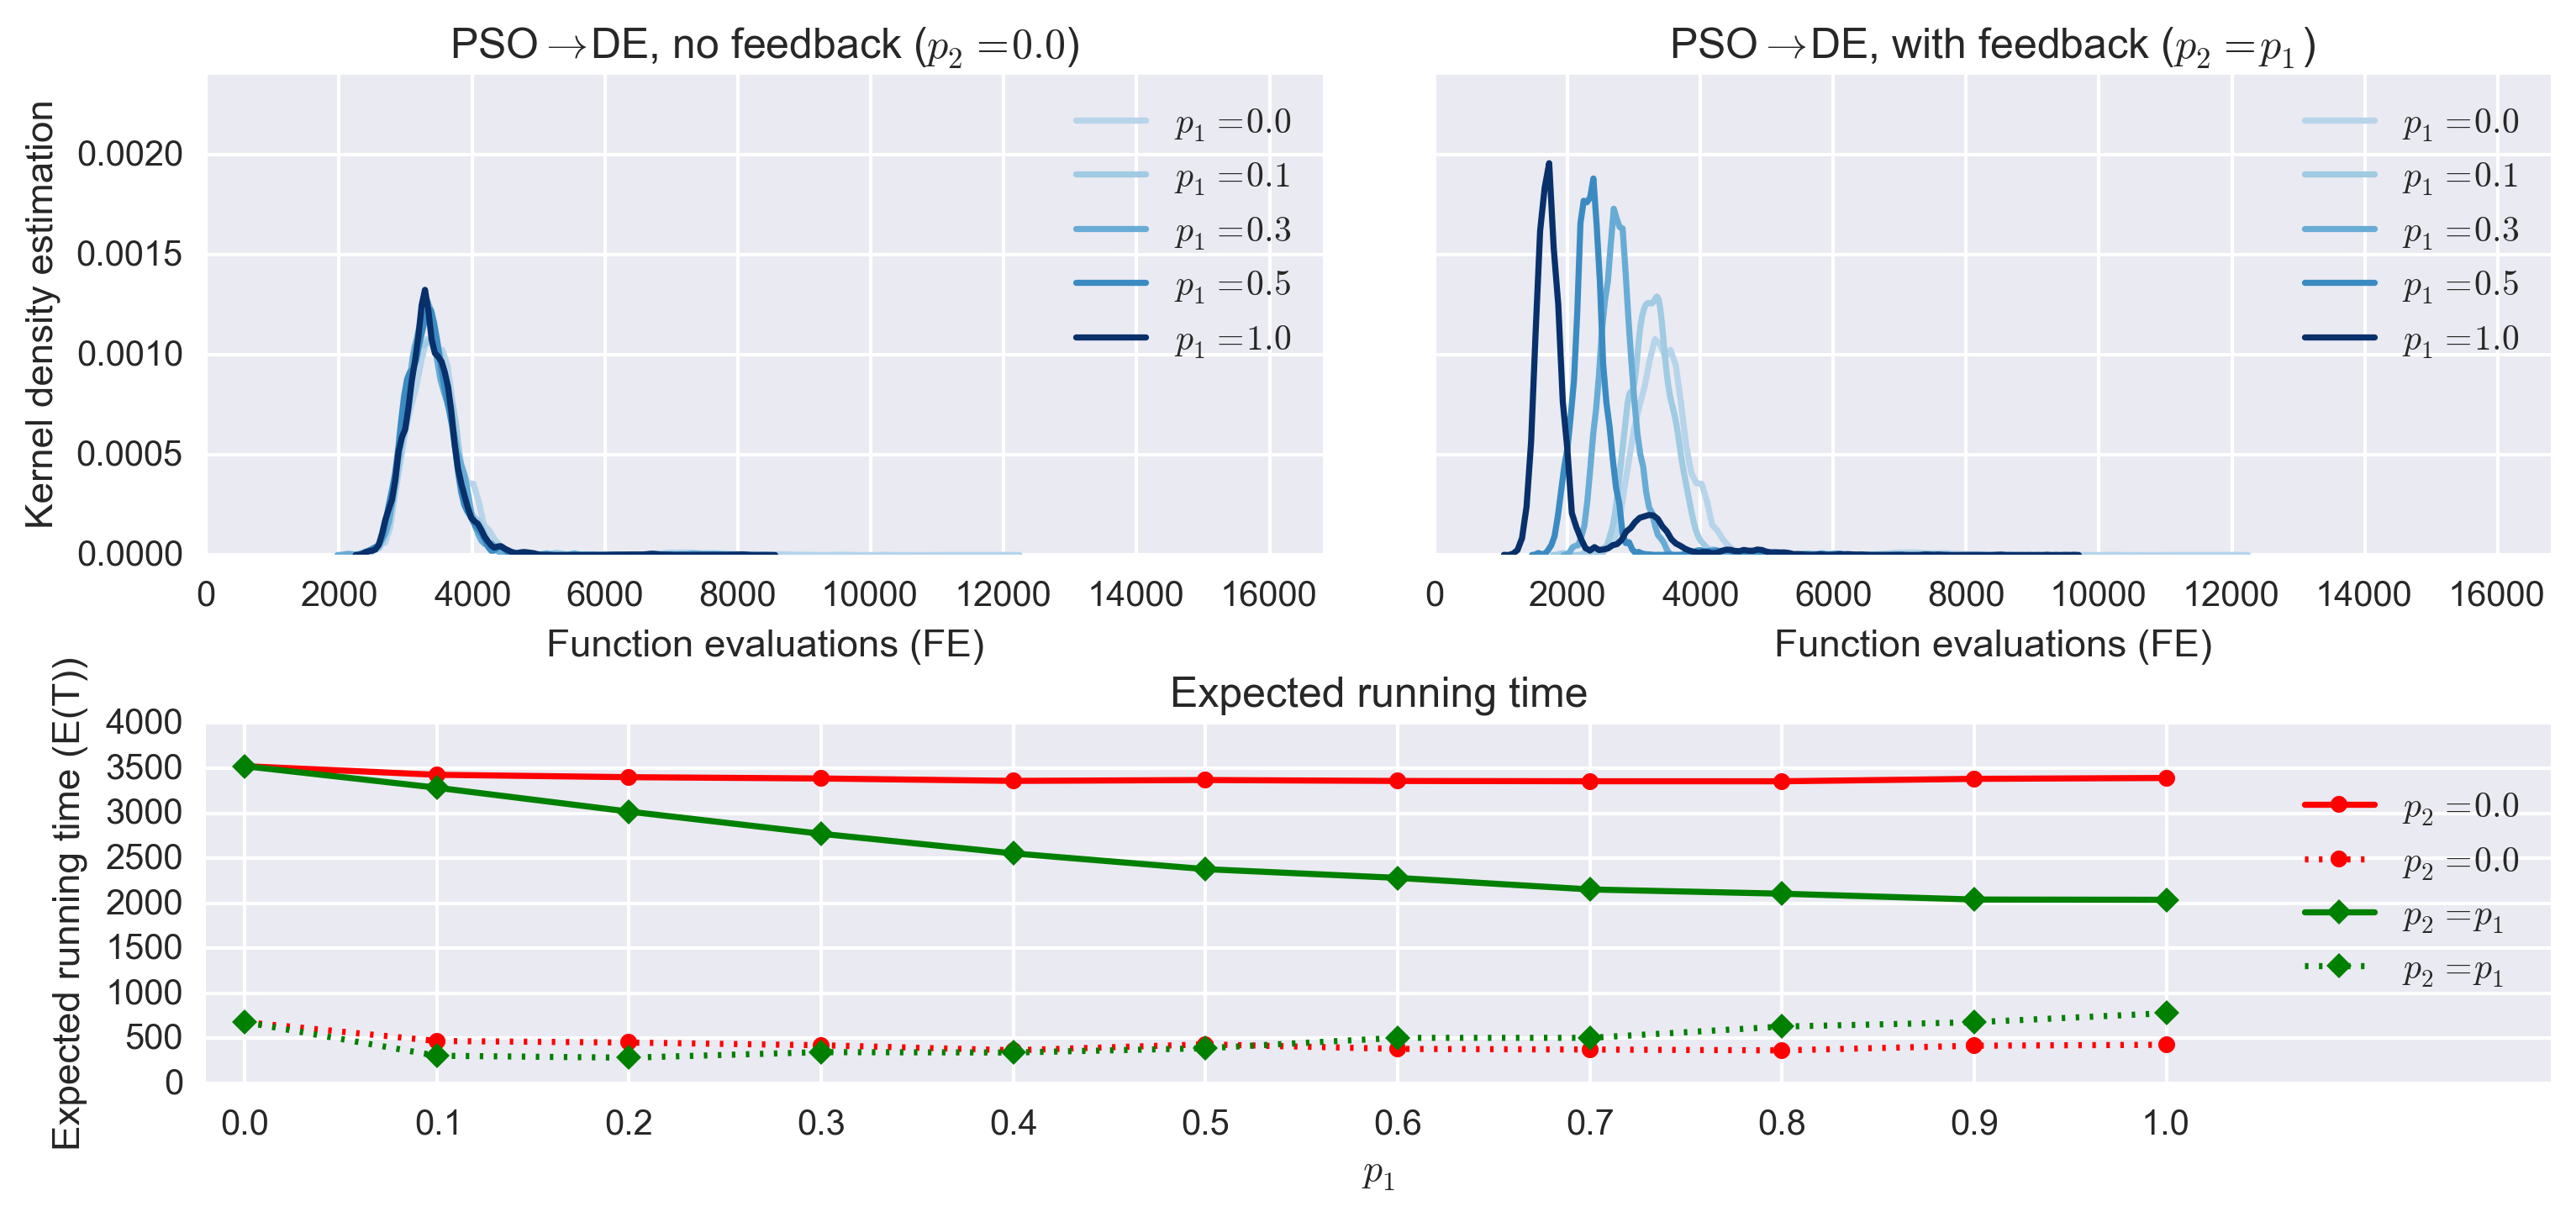
\includegraphics[width=\columnwidth]{figures/single_pso_jde_cec_7.png}
  \label{fig:single_pso_jde_7}
 \caption{Running time behaviour of homogeneous 2--island DE/DE setup on problem $f_{12}$.}
\end{figure}
Since PSO has been shown to be much slower on this problem, the difference in the expected runtime for $p_2=0$ over varying $p_1$ is almost non--existent, while for $p_1=p_2$ we see a gradual ``recovery'' from $3,500$ to $2000$ function evaluations, which was the best expected running time of DE/DE setup.

This leads us to the following observations:
\begin{enumerate}
    \item One--directional migration from $H_1$ can overall improve the performance of the $H_2$ (receiving algorithm) when the algorithm on $H_1$ is faster.
    \item Feedback to the ``better'' algorithms has an overall benefit
    \item Sending information to the ``worse'' algorithm, can 
\end{enumerate}

In the remainder of this section, and the following sections we will provide a similar analysis over several different algorithms for $H_1$, as well as larger number of problems.

For $H_1 =\mbox{DE}, H_2=\mbox{DE}$ and problems $f_1, f_4, f_6, f_7, f_9$ and $f_{13}$, we observe a very similar pattern: any migration is beneficial, with feedback significantly improving the overall running time with the increasing probability of migration.
Situation changes for more difficult multi--modal problems -- $f_{12}, f_{15}$ and $f_{16}$.
For problems $f_{12}$ (Rastrigin) and $f_{16}$ (Katsuura) migration with feedback is still more beneficial yet full--migration is not the best strategy, while for problem $f_{15}$ (Schwefel) it is the one--directional case that achieves the lowest expected running time.
SHOW SOME PLOTS HERE

The case $H_1 = \mbox{PSO}, H_2=\mbox{DE}$ exhibits similar patterns to the previous case, except that absolute expected running times are much lower due to PSO being significantly slower on each of those problems.
For that reason the migration in one--directional setup has much a lesser effect on the running time SEE(pso jde cec 1).
However, when $p_2 = p_1$ we notice that the running time of DE ``recovers'', even
Another surprising 
Another implication of 
Another important fact is thatIt is worth noting yet another benefit of the feedback: 

%This result motivates us to consider not only ``fully--connected'' topologies -- even in cases where one might think that better-suited algorithms might not benefit from the solutions from ``slower'' algorithms -- but also explore the space of asymmetrical migration parameters, i.e. $p_1 \neq p_2$.

\subsection{Varied migration experiment}

This section covers the methodology and the results of our main experiment, which extends the previous setup by allowing parameters $p_1$ and $p_2$ to have distinct values from $\{0.0, 0.1, \ldots, 1.0\}$, and test our setup on six different pairs of algorithms.
Additionally, we will monitor the stopping criteria and the number of function evaluations at the scope of the archipelago.

\begin{figure}[ht!]
    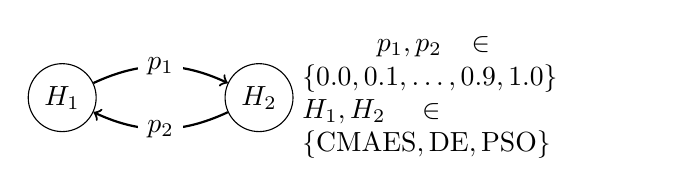
\begin{tikzpicture}[scale=2.5]
    \tikzstyle{vertex}=[draw,text=black,auto=left,circle,fill=white,minimum size=24pt]
    \tikzstyle{vertexred}=[draw,text=black,auto=left,color=red,circle,fill=white,minimum size=15pt]
    \tikzstyle{weight} = [fill=white]
    \tikzstyle{edge} = [draw,thick,->]
    \tikzstyle{edge2} = [draw,thick,-]

    \node[vertex] (a) at (0, 0) {$H_1$};
    \node[vertex] (b) at (1, 0) {$H_2$};


    \node[text width=4.4cm] at (2.1, 0.0) {%$H = \{\mbox{DE}, \mbox{CMAES}\}$\\
        $\;\;\: p_1,p_2 \in \{0.0, 0.1, \ldots, 0.9, 1.0\}$\\
        %$p_2 = \{0.0, 0.1, \ldots, 0.9, 1.0\}$\\
        $H_1,H_2 \in \{\mbox{CMAES},\mbox{DE},\mbox{PSO}\}$};

    \path[edge] (a) to[bend left=25] node[weight]{$p_1$} (b) ;
    \path[edge] (b) to[bend left=25] node[weight]{$p_2$} (a);

    \end{tikzpicture}
    \label{graph:twoisl}
    \caption{Two--island setup with heterogeneous algorithms and non--symmetrical migration probabilities.}

\end{figure}
%One might be tempted to continue with the ``local'' analysis for non--uniform migration probabilities and then extend this reasoning to a global scale -- if both islands are synchronized, and we terminate the execution as soon as \emph{any} algorithm finds the solution within global optimum, it is then an equivalent process to sampling a run from each individual island distributions $A$, $B$, and assume the number of total function evaluations (at the archipelago scope) as: FE$ = \mbox{min}(\Call{Sample}{A}, \Call{Sample}{B})$.
%We decide against it as the process get more complicated on difficult multi--modal and introduce the restarts mechanism.
%For that reason, we will monitor the stopping criteria and the running time distribution across the whole setup, and use the 
Since we extend our experiment to a wider range of problems that vary in difficulty, we expect the stopping criteria to detect the condition of convergence to suboptimal solution.
In such case, a practitioner would proceed the optimization by restarting the algorithm as long as the budget is not yet exhausted.
We embed this idea in our setup by using a boostrap resampling technique, as presented in Algorithm~\ref{alg:resample}.

%In real budget--constrained scenario, a practitioner would try to detect the third case by analyzing the convergence rate and diversity in the population and restart given algorithm with random initial conditions as long as the budget permits it.
%We allow for such operation, by employing a resampling technique, using which we construct a ``trial'', i.e., a sequence of runs among which the solution is found, or the budget is definitely exhaused (see Alg.~\ref{alg:resample}).

\begin{algorithm}
\caption{Resampling pool of runs $R$ within budget $B$}
\label{alg:resample}
\begin{algorithmic}[1]
    \Function{Resample}{$R, B$}%\Comment{Pool $M$ and budget $B$}
    \State $B' \gets 0$\Comment{Trial budget}
    \State $f' \gets \infty$\Comment{Trial objective function value}
    \Do
        \State $f, n \gets \Call{SampleRun}{R}$%\Comment{Objective value $f$ and number of function evaluations $n$}
        \State $B' \gets \mbox{max}(B' + n, B)$
        \State $f' \gets \mbox{min}(f', f)$
        \DoWhile{$B' < B \mbox{ and } (f' - f_{opt}) > 10^{-8}$}\Comment{Stop building a trial after budget is exhausted or found optimal solution}
    \EndFunction \mbox{ and }\Return $f', B'$
\end{algorithmic}
\end{algorithm}

To assess the performance of our setup we use the measure of expected number of function evaluations as proposed by Auger and Hansen in~\cite{Hansen05performanceevaluation}:

\begin{equation}
    \widehat{\mathbb{E}(T)} = \left(\dfrac{1 - \widehat{p_s}}{\widehat{p_s}}\right) B + \widehat{\mathbb{E}(T^s)},
\end{equation}
where $B$ is the allocated budget, $\widehat{p_s}$ is the estimated probability of successful run and $\widehat{\mathbb{E}(T^s)}$ is the estimated number of function evaluations of successful runs.


\subsection{Taxonomy of expected running time patterns}

When analyzing the results of our experiment we can clearly see a distinction between the unimodal ($f_1$ and $f_4$) and ``easy'' multi--modal problems ($f_6, f_7$ and $f_9$) when compared with difficult multi--modal problems ($f_{12}, f_{15}, f_{16}$ and $f_{20}$).
\begin{figure}[ht!]
\centering
\subfigure[t][Migration plays little role, and is harmful after certain threshold]{
    \label{tax:tax1}
    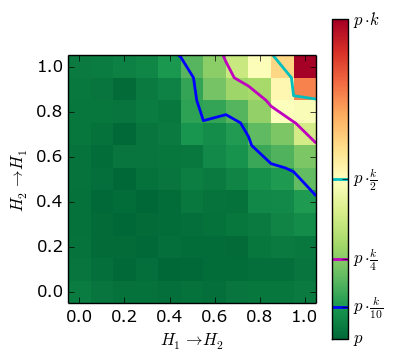
\includegraphics[width=0.45\columnwidth]{figures/taxonomy_cmaes_cmaes_cec_4.png}
}\quad
\subfigure[t][Migration has a gradual beneficial effect]{
    \label{tax:tax2}
    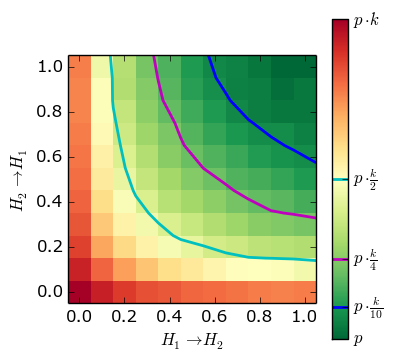
\includegraphics[width=0.45\columnwidth]{figures/taxonomy_jde_jde_cec_4.png}
}\quad
\subfigure[t][Migration starts to be beneficial after certain threshold]{
    \label{tax:tax3}
    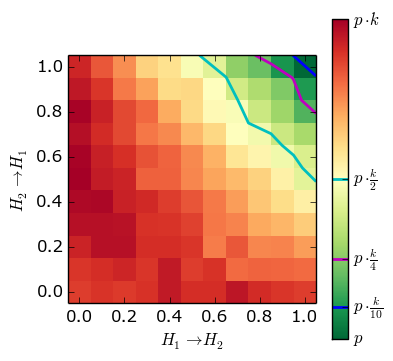
\includegraphics[width=0.45\columnwidth]{figures/taxonomy_cmaes_jde_cec_1.png}
}\quad
\subfigure[t][Migration has beneficial effect for only one parameter]{
    \label{tax:tax4}
    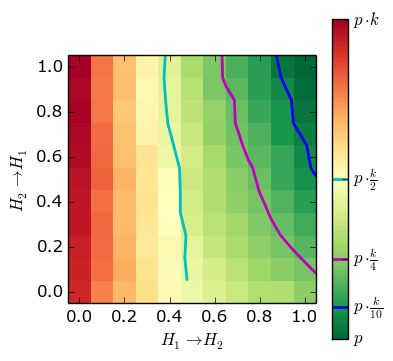
\includegraphics[width=0.45\columnwidth]{figures/taxonomy_cmaes_jde_cec_6.png}
}
\caption{Most frequent pattern of expected running times for problems $f_1$ -- $f_9$. Value $p$ is the minimal $E(T)$ within the parameter space of $p_1$ and $p_2$, while $k$ is a scaling factor between $p$ and the maximum of $E(T)$.} %Expected running time behaviour of 2--m/2--i setup on $f_{4}$ problem.}
\end{figure}
Figure~\ref{fig:jde_pso_6} presents the most typical expected running time (ERT) patterns for the unimodal, and ``easy'' multi--modal problems.
Since the exact number of function evaluations vary depending on the problem and the pair of algorithms, we present each plot as a linear progression of ERT dependent on the migration parameters from the minimal value $m$, to its maximal value represented as $m$ times a scaling factor $k$, where $k = \frac{E(T)_{max}}{E(T)_{min}}$.
In table~\ref{table:pkvalues} we provide the values for $m$ and $k$ for each pair of algorithms.
An interesting metric might be the area in the space of parameters $p_1$ and $p_2$ where $E(T)$ does not exceed $10\%$ from the $E(T)_{min}$, e.g. area where algorithms are expected to perform no worse than $10\%$ from the best parametrization available.
This can be computed as follows:
$$
m \cdot 1.1 = m \cdot k \cdot s \Rightarrow s = \frac{1.1}{k},
$$
e.g., for $k=2.0$ we have $s=0.55$, thus we can expect the area of interest to lie between the contours $m \cdot0.4 k$ and $m \cdot 0.6 k$.

%\begin{table*}
%    \label{table:pkvalues}
%    \begin{tabular}{|c|c|c|c|c|c|c|c|c|c|c|c|c|}
%        %\cline{2-3}
%        \hline
%        \multirow{3}{*}{Problems} & \multicolumn{12}{c}{$H_1$/$H_2$ on pattern~\ref{tax:tax2}} \\\hline
%         & \multicolumn{2}{c|}{CMAES/CMAES} & \multicolumn{2}{c|}{DE/DE} & \multicolumn{2}{c|}{PSO/PSO} & \multicolumn{2}{c|}{CMAES/DE} & \multicolumn{2}{c|}{DE/PSO} & \multicolumn{2}{c|}{CMAES/PSO} \\\hline
%                &   p      & k    &   p      & k    &     p      & k    &   p      & k    &    p      & k    &    p      & k \\\hline
%            1   &   1256.0 & 1.12 &   1243.0 & 1.07 &     2292.0 & 1.08 &   1293.0 & 1.51 &    2448.0 & 1.59 &    3797.0 & 3.17 \\
%            4   &   2048.0 & 1.37 &   2056.0 & 1.08 &     4118.0 & 1.03 &   2414.0 & 1.68 &    6666.0 & 2.14 &        inf & nan \\
%            6   &   1490.0 & 1.17 &   1368.0 & 1.27 &     2754.0 & 1.19 &   1583.0 & 1.78 &    3431.0 & 1.77 &     9378.0 & 3.1 \\
%            7   &   3958.0 & 2.11 &   3354.0 & 1.45 &     6454.0 & 1.73 &   4114.0 & 1.58 &    7273.0 & 1.84 &   10374.0 & 2.94 \\
%            9   &   3233.0 & 1.67 &   3054.0 & 1.33 &     6043.0 & 1.56 &   3486.0 & 1.78 &     6823.0 & 1.9 &   11552.0 & 2.78 \\
%            12  &   2872.0 & 1.67 &   2542.0 & 1.34 &     5972.0 & 1.71 &   3355.0 & 1.35 &     6932.0 & 1.4 &   13396.0 & 1.42 \\
%            13  &   3262.0 & 1.81 &   2681.0 & 1.33 &     4727.0 & 2.15 &   2783.0 & 1.42 &    4947.0 & 1.68 &    6734.0 & 2.42 \\
%            15  &   8573.0 & 2.79 &  11229.0 & 2.38 &    26044.0 & 2.41 &  18511.0 & 1.57 &    36140.0 & 1.4 &   50180.0 & 1.75 \\
%            16  &    7208.0 & inf &   9112.0 & 7.35 &   21759.0 & 26.49 &   39029.0& 2.6 &  33553.0 & 11.48 &   150652.0 & inf \\
%            20  &  351187.0 & inf &  27360.0 & 2.23 &  98133.0 & 193.94 &  20308.0 & 3.09 &   45173.0 & 3.01 &  92926.0 & 12.59 \\
%        %\hline
%    \end{tabular}
%\end{table*}


\begin{table*}
    \label{table:pkvalues}
    \begin{tabular}{|c|c|c|c|c|c|c|c|c|c|c|}
        \hline
        Seeder & $f_1$      & $f_4$ & $f_6$ & $f_7$ & $f_9$ & $f_{12}$ & $f_{13}$ & $f_{15}$ & $f_{16}$ & $f_{20}$ \\\hline
        CMAES  & N           & $f_4$ & $f_6$ & $f_7$ & $f_9$ & $f_{12}$ & $f_{13}$ & $f_{15}$ & $f_{16}$ & $f_{20}$ \\
        DE     & O (0.3)     & $f_4$ & $f_6$ & $f_7$ & $f_9$ & $f_{12}$ & $f_{13}$ & $f_{15}$ & $f_{16}$ & $f_{20}$ \\
        PSO    & B (1.0)     & $f_4$ & $f_6$ & $f_7$ & $f_9$ & $f_{12}$ & $f_{13}$ & $f_{15}$ & $f_{16}$ & $f_{20}$ \\
    \end{tabular}
\end{table*}

\begin{figure*}[htp]
  \centering
  \subfigure[Correlation between the migration probabilities and expected runnig time.]{
  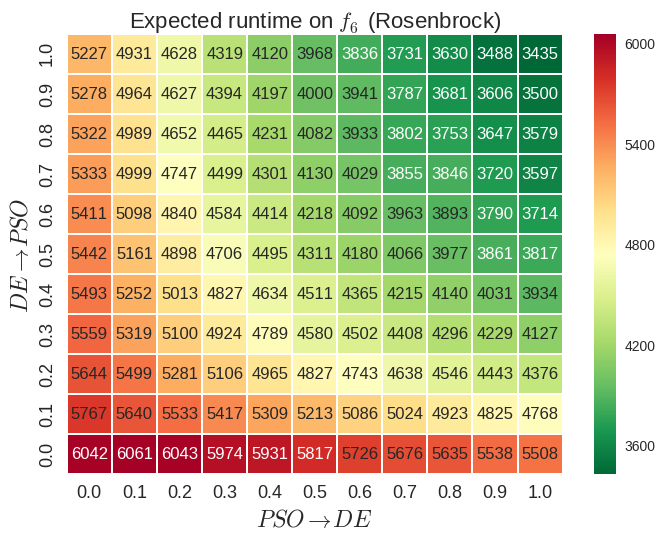
\includegraphics[width=\columnwidth]{figures/jde_pso_cec_6_0.png}
  %\includegraphics[scale=0.38]{image1}
  }\quad
  \subfigure[Distribution of $1,000$ runs (left) and $10,000$ resampled trials for $P(DE\rightarrow DE)=0.0,  0.2$ and $1.0$.]{
  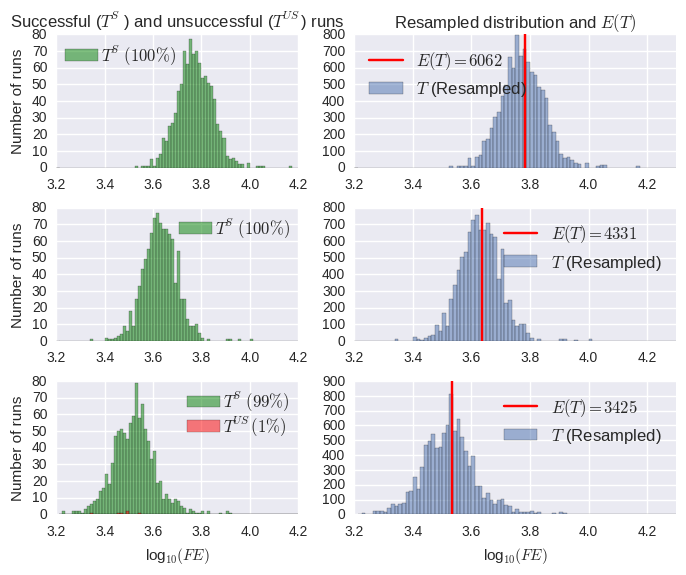
\includegraphics[width=\columnwidth]{figures/hist3_jde_pso_cec_6.png}
  }
  \label{fig:jde_pso_6}
 \caption{Running time behaviour of homogeneous 2--island DE/DE setup on problem $f_{12}$.}
\end{figure*}

In this section we provide a qualitative analysis of migration effects on the performance of our two-island model.
Due to space constraints we will restrict ourselves to reporting several most interesting cases.

\begin{figure*}[htp]
  \centering
  \subfigure[Correlation between the migration probabilities and expected runnig time.]{
  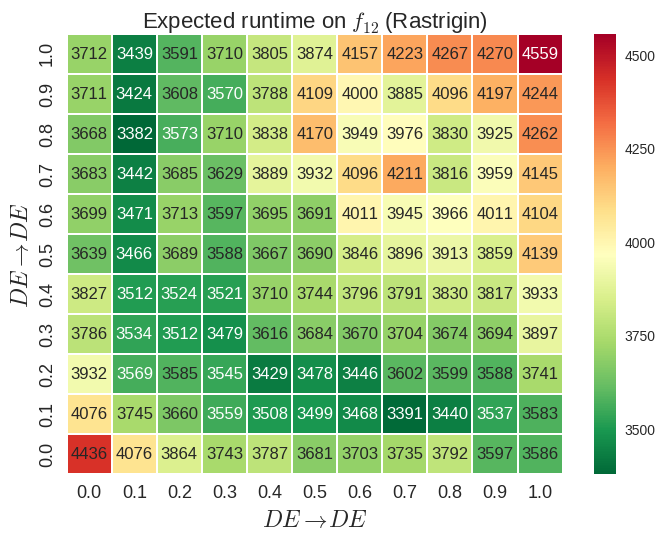
\includegraphics[width=\columnwidth]{figures/jde_jde_cec_12_0.png}
  }\quad
  \subfigure[Distribution of $1,000$ runs (left) and $10,000$ resampled trials for $P(DE\rightarrow DE)=0.0,  0.2$ and $1.0$.]{
  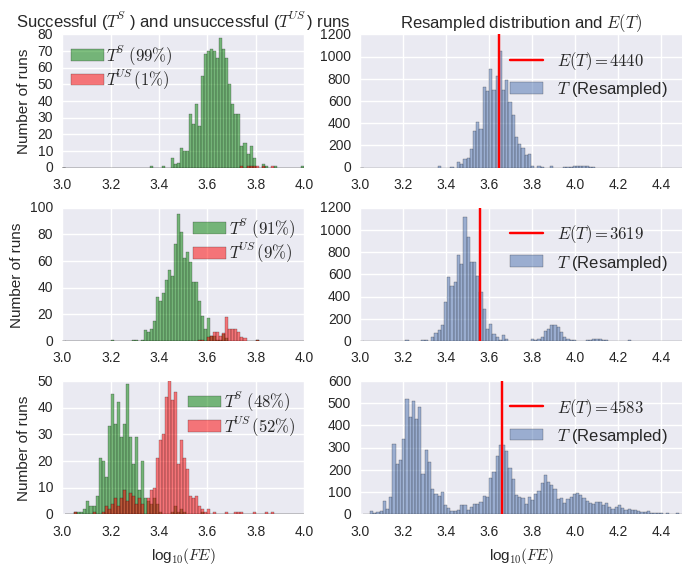
\includegraphics[width=\columnwidth]{figures/hist2_jde_jde_cec_12.png}
  }
 \caption{Running time behaviour of homogeneous 2--island DE/DE setup on problem $f_{12}$.}
\end{figure*}


In all of the homogeneous cases, we observe a symmetrical relation between the $p_1$ and $p_2$, although not always the identical one.
In this section we take a closer look at one of the expected running time patterns and provide insight on the effect of migration probability.
Let us look at the 2--metaheuristic, 2--island setup, where each island was assigned the same copy of the search algorithm.

%\begin{figure}[ht!]
%\centering
%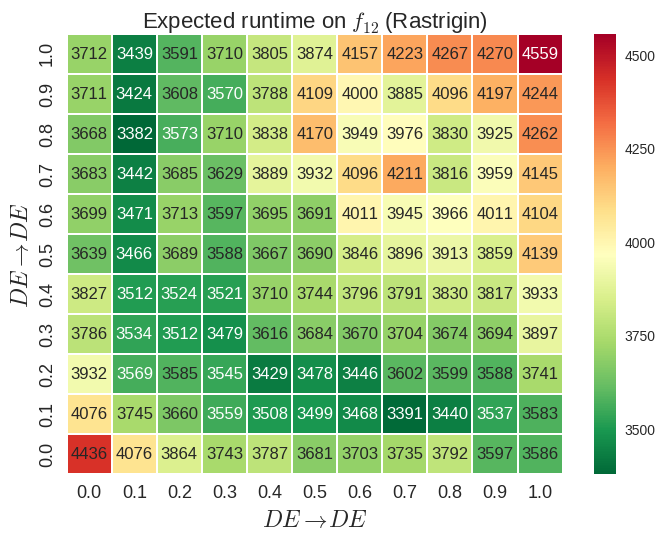
\includegraphics[width=\columnwidth]{figures/jde_jde_cec_12_0.png}
%\caption{Expected running time behaviour of 2--m/2--i setup on $f_{12}$ problem.}
%\end{figure}


%\begin{table*}
    \begin{tabular}{|l|r|r|r|r|r|r|}
    \hline
    Problem &  CMAES &  CMAES/JDE &  CMAES/PSO &  JDE/JDE &  JDE/PSO & PSO/PSO \\\hline
    $f_{1}$   &         1256 &       \textbf{1243} &       2292 &     1293 &     2448 &  3797 \\\hline
    $f_{4}$   &         \textbf{2048} &       2056 &       4118 &     2414 &     6666 &  $\infty$\footnote{Did not finish} \\\hline
    $f_{6}$   &         1490 &       \textbf{1368} &       2754 &     1583 &     3431 &  9378 \\\hline
    $f_{7}$   &         3958 &       \textbf{3354} &       6454 &     4114 &     7273 &  10374 \\\hline
    $f_{9}$   &         3233 &       \textbf{3054} &       6043 &     3486 &     6823 &  11552 \\\hline
    $f_{12}$  &         2872 &       \textbf{2542} &       5972 &     3355 &     6932 &  13396 \\\hline
    $f_{13}$  &         3262 &       \textbf{2681} &       4727 &     2783 &     4947 &  6734 \\\hline
    $f_{15}$  &         \textbf{8573} &      11229 &      26044 &    18511 &    36140 &  50180 \\\hline
    $f_{16}$  &         \textbf{7208} &       9112 &      21759 &    39029 &    33553 &  150652 \\\hline
    $f_{20}$  &       351187 &      27360 &      98133 &    \textbf{20308} &    45173 &  92926 \\\hline
    \end{tabular}
\end{table*}


%\begin{figure}[ht!]
%\centering
%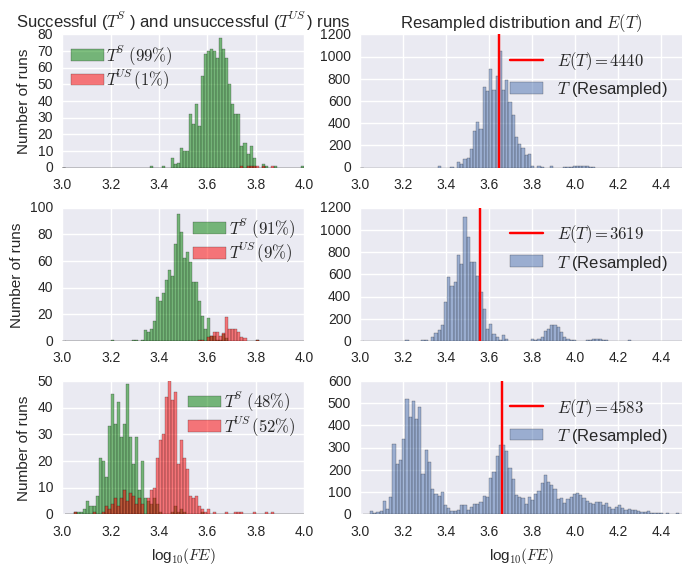
\includegraphics[width=\columnwidth]{figures/hist2_jde_jde_cec_12.png}
%\caption{}
%\end{figure}

\section{Conclusions}

\bibliographystyle{abbrv}
\bibliography{bib}

\end{document}
